\section{Systematic uncertainties}
\label{sec:kstmm:sys}

Systematic effects which may affect the angular analysis are considered if there is an effect on 
the \kpimm invariant mass distribution, the \qsq spectrum or the angular distributions.
These include the acceptance correction method and the model for the \Bd mass spectrum.
There are three main categories of sources of systematic uncertainty, listed in order of importance
\begin{itemize}
\item Any systematic bias originating from the acceptance correction method.
\item The uncertainty on the data-simulation corrections used in the acceptance correction.
%\item The uncertainty on the acceptance correction due to the limited simulation events in the high \qsq region.
\item The uncertainty on the exact parametrisation of the \Bd mass spectrum and the use of polynomials to model the angular background.
\end{itemize}
All these effects were considered for both analyses but the exact size and specific systematic effects arising from the 
data-simulation corrections and acceptance method differ between the two analyses.
An additional source of systematic uncertainty was considered for the 1.0\invfb analysis from possible peaking backgrounds.
%This is due to the improved understanding of the detector after data-taking in 2011 was completed and the different methods used.


\subsection{Systematic contributions for the 0.38\invfb analysis}

The dominant systematic for the 0.38\invfb analysis comes from the acceptance correction, with other systematic contributions 
originating from the data-simulation corrections and a minor contribution from the model used for the \Bd mass distribution.

\subsubsection{Acceptance correction}

The systematic uncertainty from the acceptance correction method comes from the choice of the radius of the hyperspheroid.
The size of the possible bias was tested by using a smaller radius (0.01) and a larger radius (0.03) then the one chosen (0.02) to select events. 
Apart from the difference in the overall statistical error on the acceptance correction weight, no significant difference was found in the absolute efficiency.
The estimates of the systematic uncertainty arising from the various data-simulation corrections were propagated 
to give an overall uncertainty for the weight value given to each event.

In order to explore possible extreme systematic variations, two methods of altering the angular analysis were tested.
Firstly, the acceptance correction was ignored and the central values of \AFB and \FL 
 were found to move less than the statistical uncertainty on the observable. 
Secondly, the background model was assumed to be flat in the \ctl and \ctk to similar effect.
These extreme changes are not propagated to the final systematic uncertainty.

The systematic error on the observables is around $\approx30\%$ of the final statistical error.
%This contributes an $\approx3-4\%$ addition to the error in quadrature.
When added in quadrature to the statistical error, this only makes the total error (3-4)\% larger.
This is with the exception of the highest \qsq bin where 
the low simulation statistics leads to the total error being 10\% larger than the statistical error.


\subsubsection{Data-simulation corrections}

A conservative estimate of the uncertainty based on smearing the IP of the simulated tracks was tested by using the unsmeared tracks.
This can change the efficiency to select the events and the calculated angles.
%The gives an overall change to the total efficiency of \textcolor{red}{XX} and a change in the angular distribution of \textcolor{red}{YY}`.
A conservative estimate of the uncertainty associated with applying the correction for the hadron particle identification
 was evaluated by using the simulated values instead of the data-derived values.
This estimate gives a change in the absolute efficiency of around 20\% but does not change the angular distributions.
This estimate of the systematic uncertainty for the relative efficiency of the muon identification was obtained by changing the relative efficiency by one standard deviation.
The weight applied to the simulation is shifted down by $1\sigma$ for $p_\mu < 10\gevc$ and upwards for $p_\mu>10\gevc$.
A similar procedure is used to gain an estimate of the relative tracking efficiency but changing the weight applied for track momenta above and below 20\gev.
The effect of these changes on the measurement of the differential branching fraction is much smaller as it cancels out in the normalisation to \BdToJpsiKstar to first order.

\subsubsection{Mass model}

The systematic uncertainty associated with the model of the \Bd mass spectrum is evaluated by
 replacing the double Gaussian function with a double Crystal Ball function.
This tests the degree to which the tails of the Gaussian distribution are correctly modelled.
The systematic uncertainty associated with the background model is checked by using a linear function instead of an exponential function.
This is because the upper mass sideband may contain unknown background which can be incorrectly modelled by using a falling exponential.
The systematic uncertainty associated with using a polynomial to model the angular background is checked by
using a template function for the background, taken from a fit to the \Bd upper mass sideband, i.e. events with \mB of greater then 5400\mevmevcccc.
This ensures that the background model is free of any signal contribution but assumes that the high mass background is entirely combinatorial 
and the angular distribution is equivalent under the signal peak and in the high mass region.


\subsection{Systematic contributions in the 1.0\invfb analysis}

The contributions to the systematic uncertainty on the angular analysis of 1.0\invfb come from the 
the event selection, the model for the \Bd invariant mass and the acceptance correction.
The dominant effect comes from both the acceptance correction and the data-simulation corrections.
Tables of the size of the contribution from each of the possible sources of systematic uncertainty are given in Appendix~\ref{app:kstmm:systematics}.

\subsubsection{ Acceptance Correction}


The systematic uncertainty on the acceptance correction method was estimated by testing the addition
 of both factorisable effects, testing the addition of  non-factorisable effects and by using a different \qsq binning scheme.
The systematic uncertainty associated with factorisable effects was tested by changing the 
acceptance correction weight by a factorisable function that increases the weight at extreme values of 
\ctl and \ctk,
\begin{align}
\omega_i \to \omega_i \times ( 1 + \alpha \ctl^2 ) \times ( 1 + \alpha \ctk^2 ) .
\end{align}
The value of $\alpha$ was chosen to give a 10\% increase in the weight values at the extremities of the 
angular distribution. 
The estimate includes any mis-modelling of the efficiency in such a way that it will maximally affect the angular distribution.
The systematic uncertainty associated with non-factorisable effects was tested as described in Sec.~\ref{sec:kstmm:facac:nonfac}.
A non-factorisable effect of 10\% is used to provide an estimate of any hidden systematic effect because this is the maximum value that the 
acceptance correction is insensitive to.
The estimates of the systematic uncertainty from the acceptance correction are the dominant contribution to the total systematic error.


\subsubsection{Data-simulation corrections}

An estimate of the systematic uncertainty of each of the data-simulation corrections was evaluated for each of the different corrections.
The systematic uncertainty on the trigger efficiency is estimated by applying a weight of $\pm3\%$ to events with a muon of momentum less than 10\gev.
This comes from an estimate of the L0 trigger efficiency~\cite{Aaij:2012me}.
The systematic uncertainty on the relative tracking efficiency correction is changed twice. 
The relative tracking efficiency correction is shifted firstly down by one $\sigma$ for tracks below 20\gev and up by one $\sigma$ for tracks above 20\gev
 and secondly in the opposite direction.
This correction is chosen to reflect the possibility of a systematic mis-modelling of low momentum tracks and
to reflect the relatively easier reconstruction of high momentum tracks.
The relative efficiency for the muon identification is systematically shifted using the same method as the
relative tracking efficiency, but for muons with momentum above and below 10\gevc.
A possible source of systematic uncertainty from changing the particle identification for hadrons comes from the binning scheme used to calculate the new \dll values from data.
The effect of the binning scheme is tested twice by drawing \dll values from bins higher or lower for events close to the edge of the bin boundary.

In order to introduce a very conservative source of systematic uncertainty all hadrons with a momentum of less than
 3\gevc were removed from the sample of phase space simulated events.
The effect of this cut on the weight distribution as a function of \ctk and the effect on the re-weighted phase 
space simulated events is shown in Fig~\ref{fig:kstmm:sys:hadronp}.
\begin{figure}[tbp]
\centering
%\subfigure[]{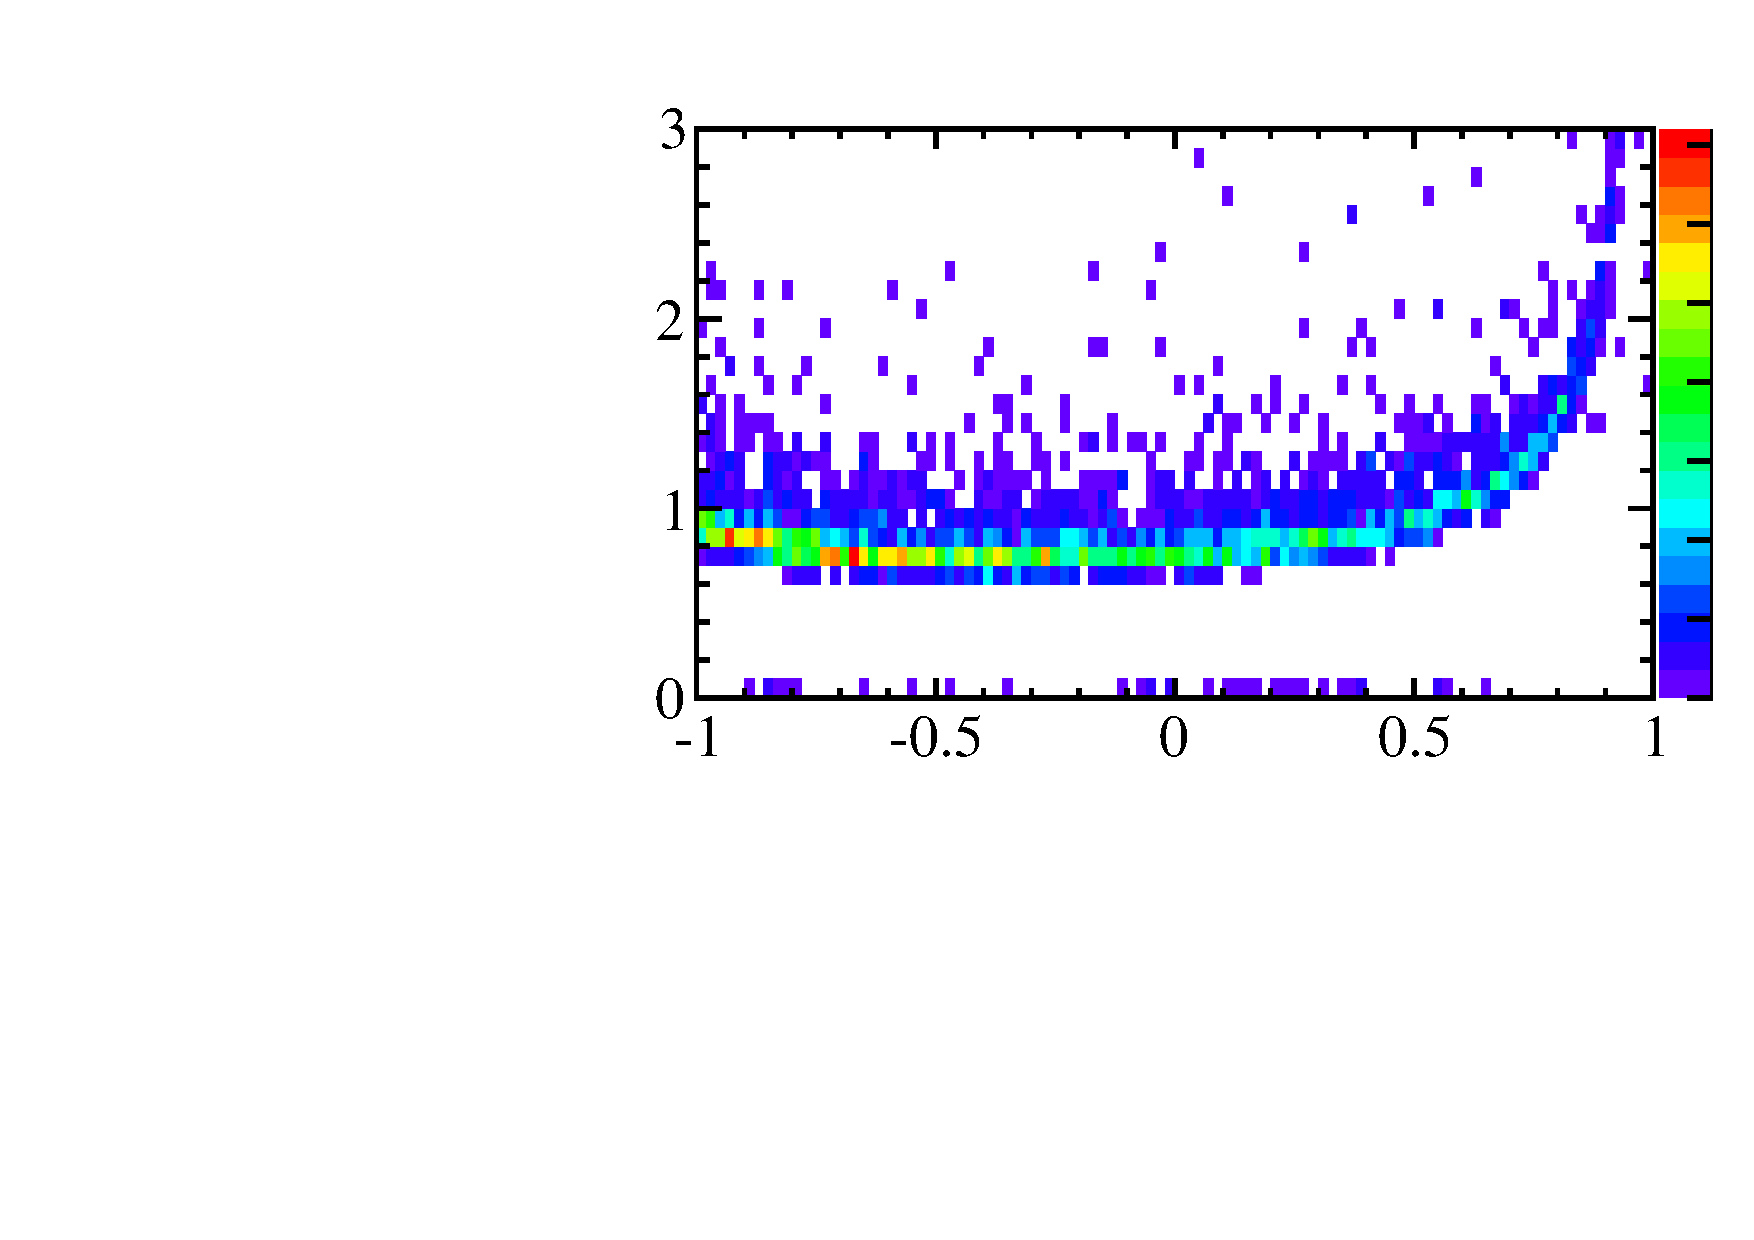
\includegraphics[width=0.48\columnwidth]{chapter5/figs/sys/validation_weight_ctk_hadronpcut.pdf}}
%\subfigure[]{
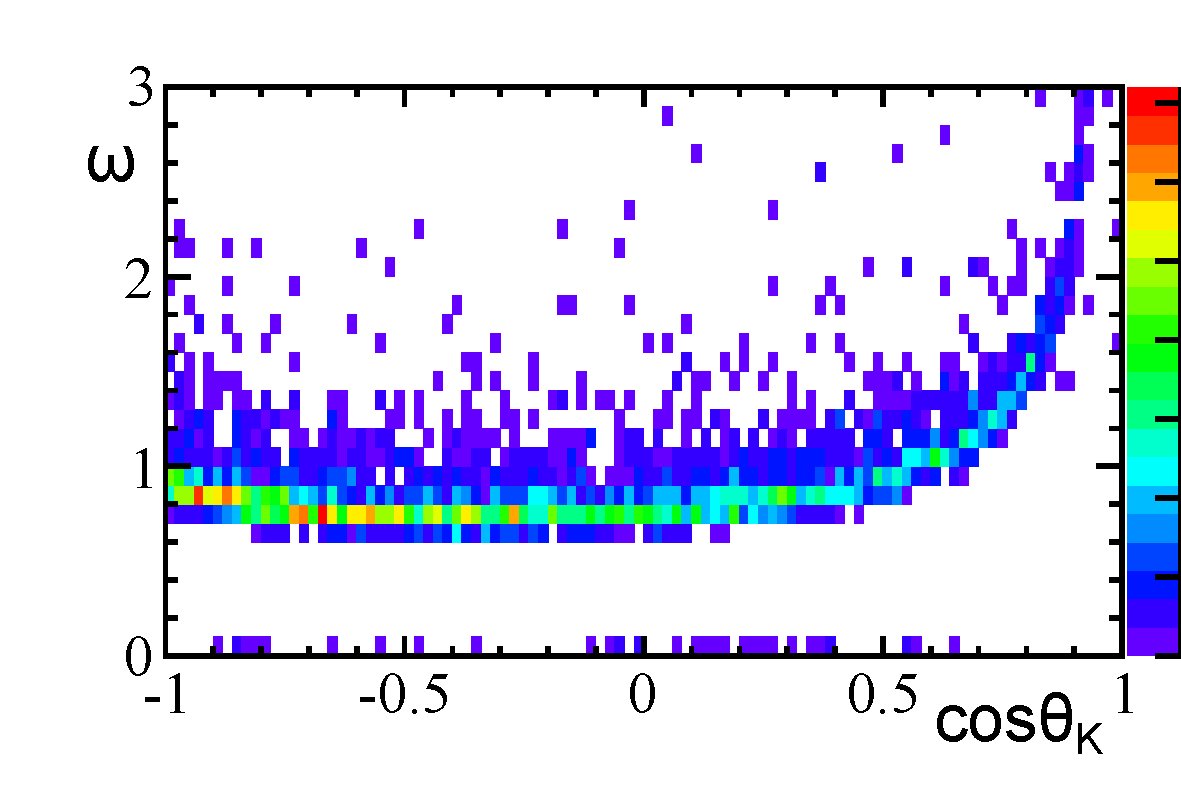
\includegraphics[width=0.48\columnwidth]{chapter5/figs/sys/validation_weight_ctk_hadronpcut_new.pdf}
%}
\caption[  The effect of the removal of all hadrons of $p<3\gevc$ from the phase space simulation used in the acceptance correction.  ]
{ The effect of the removal of all hadrons of $p<3\gevc$ from the phase space simulation used in the acceptance correction. 
%The effect on a re-weighted phase space sample is shown in (a) where 
It is possible to see the artificially higher weights at high values of \ctk. 
%The effect on the weight values on the data sample is shown in (b). 
~\label{fig:kstmm:sys:hadronp} }
\end{figure}
%The estimate of the systematic uncertainty from this cut is not propagated to the final uncertainty because it is not a realistic .

\subsubsection{Mass Model}

There is a systematic effect from using the same mass model for the multiple different \qsq bins.
The widths of the two Crystal Ball functions used for the signal mass model are checked using 
corrected simulated \BdToKstmm data. The width is found to vary within errors to $\pm5\%$ and
both widths in the signal mass model are varied by this amount to compensate for this.

The systematic uncertainty on the parametrisation of the angular background is estimated by using a 
constant background as opposed to a $2^{\text{nd}}$ order Chebychev polynomial.
This has no significant impact on the values of the angular observables.

\subsubsection{Event Selection}

The two sources of possible systematic uncertainty from the event selection are from the 
consideration of peaking backgrounds and from the treatment of multiple candidates.
Peaking background decays such as \Bs\to\Kstarz\mumu and \Bs\to\varphi\mumu are difficult to account
for in the angular fit because the angular distribution of the decay products is not well known.
A conservative estimate of the contribution from these decays is assumed by assigning a
5\% systematic to the events that have $\AFB=\pm1$, $\FL=0,1$.
This method gives a total estimate of the systematic uncertainty from peaking backgrounds of approximately 2\%.

The treatment of multiple candidates is systematically accounted for by removing all events with multiple 
candidates.
The fraction of events with multiple candidates is between 1-2\% and consists mainly of \ktopi swapped candidates.
This has no impact on the final values for the angular observables.

\subsubsection{Tables of systematic uncertainties}


